\documentclass[12pt]{article}

\usepackage[utf8]{inputenc}
\usepackage[margin=1in,footskip=0.25in]{geometry}
\usepackage[english,activeacute]{babel}
\usepackage{amsmath}
\usepackage{graphicx}
\title{Habitat Selection}
\author{Brian D. Gerber}

\begin{document}

\maketitle
\section{Habitat Selection with independent spatial locations}

Habitat selection modeling has a long history (Northrup et al. 2022). It is also fairly confusing as the terminology and understanding of the statistical modeling has evolved. From Hooten et al. 2017, "Mystery and misunderstanding surrounds the proper implementation to fitting RSF models.”\\

A common habitat selection model will use animal-borne telemetry location data. We will consider these spatially locations independent, such that consecutive locations do not depend on each other. A major part of many telemetry data is dependence due to movement constraints of the animal. For the locations to be independent, there has to have been a long enough time between locations such  that the animal could have accessed any part of the landscape that is considered available. The important word here is \textbf{could}, rather than did. Essentially, we are interested in these independent behavioral decisions of where the animal chooses to be located on the landscape that we are considering available. As part of this type of model, \textbf{we} need to decide on all the locations on a landscape that are available to the animal to choose from. This is a decision by us, but it still needs to be justified based on determining whether locations are independent. The boundary of this available area is often chosen to be the home range of the individual, but it could also be a larger landscape though. \\
The simplest habitat selection model and the one that has been historically been the most commonly used is one where we assume all locations are equally available to the individual animal within a defined area (e.g. home range). In the literature, this is the `Traditional Resource Selection Function'. We want to estimate whether animals are using certain landscape/spatial features in this area more than they are available to the animal (selection) or whether they are using these them less than they are available (avoidance). The statistical framework that combines use, selection, and availability is the weighted distribution formulation of a point process model (Hooten et al. 2017).\\

The components:

\begin{itemize}
\item $\boldsymbol{\mu}_{i}$ is a 2 x 1 vector of the animal's true geographic coordinate for relocation i (i.e., the data!).
\item $\textbf{x}(\boldsymbol{\mu}_{i})$ are the environmental/spatial features hypothesized to influence animal selection at relocation $\boldsymbol{\mu}_{i}$ (i.e., the covariates!).
\item the function g() is called the selection function and depends on $\boldsymbol{\beta} $
\item  $\boldsymbol{\beta}$ are the associated selection coefficients associated with $\textbf{x}(\boldsymbol{\mu}_{i})$
\item the function f() is called the availability function and depends on $\boldsymbol{\theta}$
\item  $\boldsymbol{\theta}$ are the associated availability coefficients 
\end{itemize}

To put this together, we can define the probability density function of the locations ($\boldsymbol{\mu}_{i}$) as,


\begin{align*}
\boldsymbol{\mu}_{i} \sim& [\boldsymbol{\mu}_{i}| \boldsymbol{\beta}, \boldsymbol{\theta}] \\
[\boldsymbol{\mu}_{i}| \boldsymbol{\beta}, \boldsymbol{\theta}] \equiv &  \frac{g(\textbf{x}(\boldsymbol{\mu}_{i}, \boldsymbol{\beta}))f(\boldsymbol{\mu}_{i},\boldsymbol{\theta})}{\int g(\textbf{x}(\boldsymbol{\mu}, \boldsymbol{\beta}))f(\boldsymbol{\mu},\boldsymbol{\theta})d\boldsymbol{\mu}}.
\end{align*}

However, we stated that we will make all locations and associated environmental/spatial features equally available to the individual within a defined area (called the support of the point process, $\mathcal{M}$). Therefore, the availability function is uniform and be removed as it would be equivalent to multiplying the selection function for each location $i$ by one. We can then simplify our model to


\begin{align*}
[\boldsymbol{\mu}_{i}| \boldsymbol{\beta}] \equiv &  \frac{g(\textbf{x}(\boldsymbol{\mu}_{i}, \boldsymbol{\beta}))}{\int g(\textbf{x}(\boldsymbol{\mu}, \boldsymbol{\beta}))d\boldsymbol{\mu}}.
\end{align*}

But what is this g function? Generally, it can be any deterministic mathematical function that has positive support. Specifically though, it is commonly defined as exponential, g() = exp(). Therefore, we can define our final model as,

\begin{align*}
[\boldsymbol{\mu}_{i}| \boldsymbol{\beta}] \equiv &  \frac{\text{exp}(\textbf{x}'(\boldsymbol{\mu}_{i}) \boldsymbol{\beta})}{\int \text{exp}(\textbf{x}'(\boldsymbol{\mu}) \boldsymbol{\beta})d\boldsymbol{\mu}}.
\end{align*}

Lastly, lets connect this model across N independent spatial points and define the complete likelihood as,

\begin{align*}
 \prod_{i=1}^{N}  \frac{\text{exp}(\textbf{x}'(\boldsymbol{\mu}_{i}) \boldsymbol{\beta})}{\int \text{exp}(\textbf{x}'(\boldsymbol{\mu}) \boldsymbol{\beta})d\boldsymbol{\mu}}.
\end{align*}

\subsection{How do we fit this model?}

It happens that we can fit this model with logistic regression. \\

\subsubsection{Data Setup}
The main idea in the logistic regression approach is to convert the individual spatial locations into a binary data set where the observed locations are represented by ones and the available locations are represented by zeros. That is, a background sample is typically taken from the availability distribution f in such a way that it represents a large but finite set of possible locations the individual could have occupied. The environmental covariates ($\textbf{x}_{i}$) at the individual locations ($\boldsymbol{\mu}_{i}$) are associated with each of the ones for i = 1,... N, and similarly, the covariates are recorded for the background sample of M- N locations. The response variable is then specified as $y \equiv (1,.....,1,0,...0)'$ and used in a standard logistic regression with the complete set of covariates. That is, the fitting model becomes $y_{i}\sim \text{Bern}(p_{i})$ where $\text{logit}(p_i) = \textbf{x}'\boldsymbol{\beta}$ for i = 1, ...., m total binary observations.

\subsubsection{Available Sample}
The background sample (the zeros of length M) is what is providing the approximation of the integral in the above formulas (i.e., denominator). It is important we have enough locations of zeros to make sure this integral is well approximated (Northrup et al. 2013). The two ways we can ensure this are that we obtain many locations in the spatial areas of interest ($\mathcal{M}$) and assign them the response of zero. The second thing we can do is weight our observations in the logistic regression model. In R and in the function glm, we can do this with weight argument. Specifically, we want to create a vector that corresponds to $y$, where we assign a 1 for each value of 1 in $y$ and a 1000 (or large number) to each value of zero in $y$. To test whether we have enough of a background sample, we can increase the number of zeros until the estimated coefficients ($\hat{\boldsymbol{\beta}}$) no longer change.

\subsubsection{Predictions}

We need to be careful when we make predictions of relative intensity of selection after we fit the logistic regression model. This is because we are using code to approximate a different model, i.e., we are not really fitting a logistic regression model. We are fitting a weighted distribution formulation of a point process model with an assumed exponential relationship for the selection function. Therefore, we do not want to blindly use functions in R that would have us use the logit-inverse link function, as this is not a logistic regression. Specifically, to predict values of relative intensity of habitat selection, we want to use the exponential function. We also do not want to use the estimated intercept when making predictions. This sounds rather odd, but the intercept does not have much of a meaning here in this model. It is primarily a function of the ratio of used to available locations. The more available locations then the smaller the intercept will be. This is not a useful parameter. Instead to make predictions, we want to combine the linear terms (without the intercept) and multiply them with the covariates of interest, sum these, and then exponentiate. Mathematically, this would be,

\begin{align*}
e^{\textbf{x}'(\boldsymbol{\mu}_{i})\boldsymbol{\beta}}
\end{align*}

\subsection{Independent relocations of one or more individual}


\begin{figure}[h!]
\centering
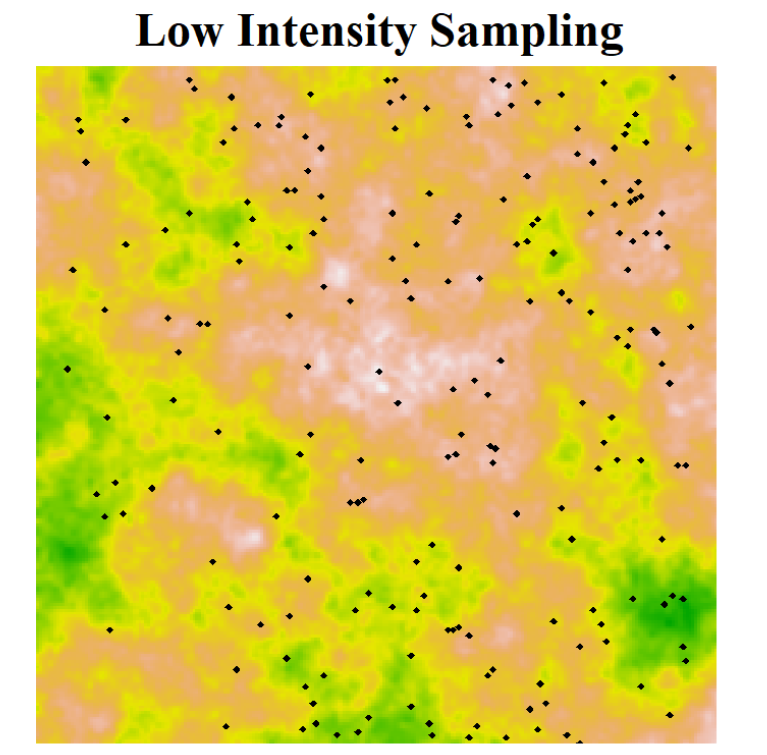
\includegraphics{sampling1.png}
\end{figure}

The relative intensity of selection is depicted by the variation in colors and each black dot is considered an independent relocation within this landscape. The entire area is considered available to the individual or individuals. 


\section{Habitat Selection with temporally dependent spatial locations}

Modern tracking technology allows us to collect high frequency relocation data on individuals. Therefore, for many species and relocation intervals (time between telemetry fixes/relocations) what is available to the animal is constrained by how the animal moves (e.g., speed and direction). Ignoring this constraint and assuming the data are independent will lead to psedureplication and thus unreliable inference. As such, we need to build this movement constraint into our habitat selection model, thereby connecting the spatial process model with a movement model. We can depict this model by defining the probability density function of the relocations and the availability distribution in terms of relocations from i-1 to i and the time between these ($\Delta_{i}$). For example, we can generally specify it as,

\begin{align*}
[\boldsymbol{\mu}_{i}|\boldsymbol{\mu}_{i-1} \boldsymbol{\beta}, \boldsymbol{\theta}] \equiv &  \frac{g(\textbf{x}(\boldsymbol{\mu}_{i}, \boldsymbol{\beta}))f(\boldsymbol{\mu}_{i}|\boldsymbol{\mu}_{i-1},\Delta_{i},\boldsymbol{\theta})}{\int g(\textbf{x}(\boldsymbol{\mu}_{i}, \boldsymbol{\beta}))f(\boldsymbol{\mu}_{i}|\boldsymbol{\mu}_{i-1},\Delta_{i},\boldsymbol{\theta})d\boldsymbol{\mu}}.
\end{align*}

\subsection{How do we fit this model?}

Commonly, this model is not fit directly, but rather we setup the data to create used (1) and available (0) samples for each step of a movement process. This is a movement-based habitat selection function or a step-selection function. We can fit this model using conditional logistic regression. Rather than the data being a vector of 0 and 1's, we match each used location (case) with a specific set of zeros (control). For each used and available, we can include covariates. We can think about this as each 1 being paired with its own specific set of zeros to estimate the relative intensity of selection while the animal is moving through the landscape. 

\subsection{Highly dependent relocations of one individual}

The relative intensity of selection is depicted by the variation in colors and each black dot is a dependent relocation within this landscape. The dependence is due to the movement dynamics of the individual, which is captured by sequential relocations in a short time period relative to the total area of the landscape. For these data, we do not want to assume that the entire landscape is available to this individual, because of the constraints on movement. Rather, we want to setup the data such that each used location is compared to neraby available locations. We decide on the available samples (and environmental covariates) for each used location based on estimating movement parameters and then sampling locations around the used location. 

\begin{figure}[h!]
\centering
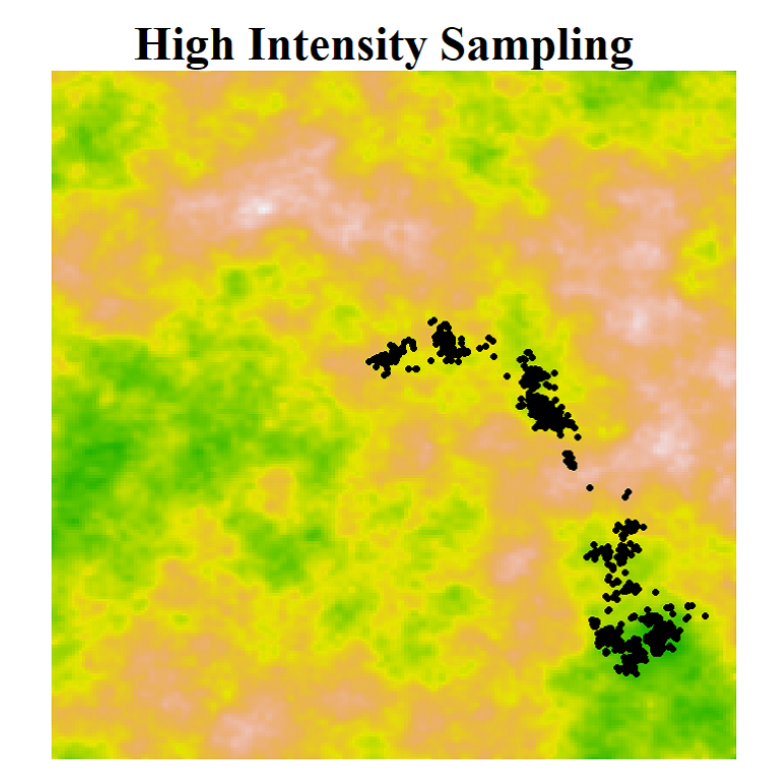
\includegraphics{sampling2.png}
\end{figure}

\pagebreak

\section{References}

\indent\indent  Hooten, M. B., Johnson, D. S., McClintock, B. T., \& Morales, J. M. (2017). Animal movement: statistical models for telemetry data. CRC press.\\

Northrup, J. M., Hooten, M. B., Anderson Jr, C. R., \& Wittemyer, G. (2013). Practical guidance on characterizing availability in resource selection functions under a use–availability design. Ecology, 94(7), 1456-1463.\\

Northrup, J. M., Vander Wal, E., Bonar, M., Fieberg, J., Laforge, M. P., Leclerc, M., ... \& Gerber, B. D. (2022). Conceptual and methodological advances in habitat‐selection modeling: guidelines for ecology and evolution. Ecological Applications, 32(1), e02470.


\end{document}